
  
  \subsection{Removing borders}
    A normal picture from the kvasir dataset, as seen earlier, has more to it than just the picture we are after.
    As mentioned over the less clutter we can get in our data the better. So one of the first thing we should do is to remove the frame.
    \begin{figure}[ht]
      \centering
      \begin{minipage}[b]{0.45\textwidth}
	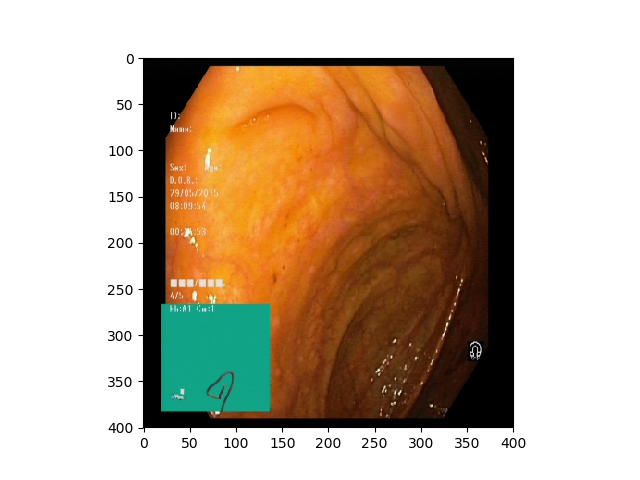
\includegraphics[width=\textwidth]{methods/figures/No_crop.png}
	\caption{Original image with no edges removed}
      \end{minipage}
      \hfill
      \begin{minipage}[b]{0.45\textwidth}
	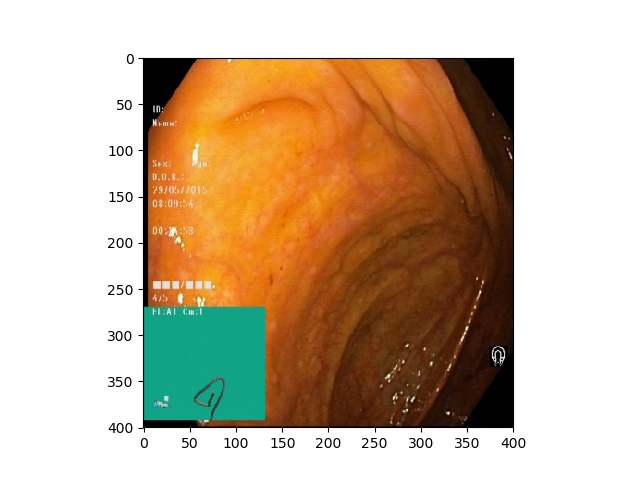
\includegraphics[width=\textwidth]{methods/figures/Crop.png}
	\caption{Edges of the image removed}
      \end{minipage}
    \end{figure}
    The biggest reason why this is done is because of the lack of information in the black, uniform pixels. Since the 
    black area differs in every image, the area is saved as a feature. This feature contains no relevant information for the analysis,
    so it is easier if it is just discarded. \\
    
    The image is cropped using 2 simple algorithms, first we run a morphological opening with a $5\times5$ kernel on a black/white copy of the image. 
    This will remove any unwanted artifacts and/or text in the black area. Now that the border is guarantied black, we can do a simple crop where the border stops.
    
    %identical
    %black beckomes a featire, with features 
    
  \subsection{Adjusting brightness and contrast}
  TODO LATER.
  
  \subsection{Removing artifacts and saturated spots}
  In addition to the border areas there are also other areas that bear little to no information. This is the bright spots where the light from the camera-pill is saturating the CCD in the pill.
  White areas like this can be treated as a feature, and as with the border, this feature contains no relevant information.
  %TODO cite Zeno Albisser
  In the article \textit{Computer-Aided Screening of Capsule Endoscopy Videos} from Zeno Albisser it is proposed a way to remove bright areas by using a horizontal gradient over the bright areas.
  In the loading of the images a similar treatment %TODO find word
  of the images is done.
  
  \subsection{Using a Contextencoder to predict image parts}
  At this point we have used naive methods to enhance the data. Another big part of the image has not been mentioned this far, and that is the green square many of the images contains.
  
  \begin{figure}[h]
    \centering
    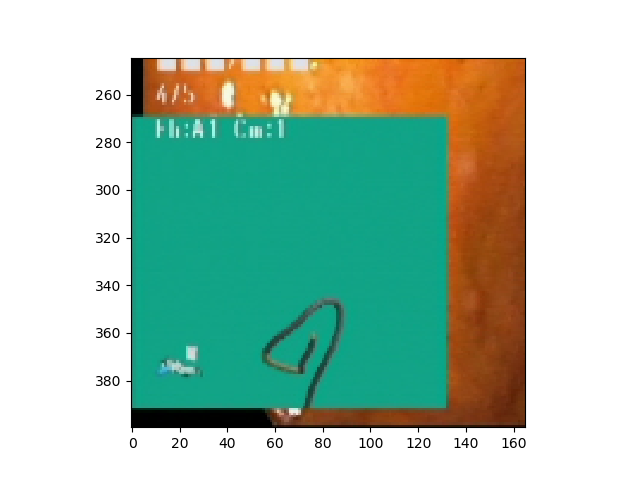
\includegraphics[scale=0.5]{methods/figures/Green_square.png}
    \caption{A typical example of a green square containing information about where in the GI-tract the image is taken from}
  \end{figure}
  
  A way to remove the square is to continue to use a naive method, perhaps with a horizontal gradient or a similar technique. 
  However we can use a convolutional neural net to try to predict what would be behind the area. 
  
  \subsubsection{Using a GAN}
  As described earlier in the thesis %TODO describe earlier
  we can use an adversarial network to generate images. 
  The general Contextencoder has three main parts: Encoder, decoder and a Discriminator.
  
  \begin{figure}[ht]
    \centering
    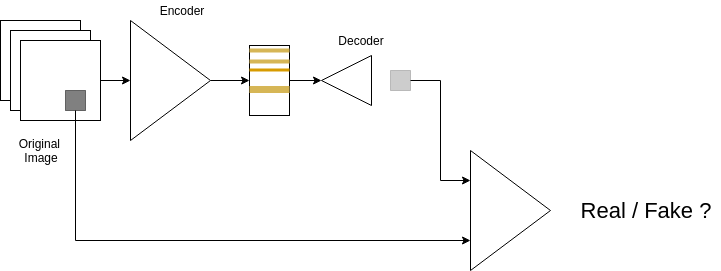
\includegraphics[scale=0.5]{methods/figures/Contextencoder.png}
    \caption{A simple Contextencoder}
  \end{figure}
  
  %TODO MENTION THAT WE ARE NOT TRAININ ON GREEN IMGS
  %TODO MENTION THAT WE ARE NOT TRAININ ON GREEN IMGS
  %TODO MENTION THAT WE ARE NOT TRAININ ON GREEN IMGS
  First an (often random) area is removed from the original image, and is stored as a copy. Then the decoder takes the reminding image and compresses it to a latent space. From there 
  the encoder tries to build a new image that is the same size as the missing peace. \\
  After the peace is made it is sent to the discriminator, together with the original peace. The discriminator takes both the generated image as well as the original image and tries to give a prediction if it
  believes if the part it got was a generated or original image.
  Training and evaluation is the same as described in the general description of how an generative adversarial network is working.
  
  \subsection{Using a Variational Autoencoder to train the adversarial network}
    This chapter talks about the use of a Variational autoencoder to train the generator.
    
    
    
  \subsubsection{Setup of the GAN}
  Using the Contextencoder described we made 3 %TODO make 2 more programs
  similar programs for image prediction.\\
  \vspace{5px}
  \textbf{Random masker:} The first program is designed to work with any data as long as you train the weights on sufficient data. The random masker trains on images where the area masked is 
  uniformly distributed throughout the images. This approach is highly general, and will give a better masking on nongreen squares, compared to the corner masker.  
  
  \vspace{5px}
  \textbf{Corner masker:} The corner masker is designed to only mask the bottom left corner where the green square is located, this means that it is better at finding the area behind the green square, but it is much 
  worse at predicting any other part of the image.
  
  \vspace{5px}
  \textbf{Categorical masker:} The categorical masker is a mix between the two prior models. The categorical masker divides the image in to 9 different equally placed squares, and only masks those areas. %TODO Is middle one removed?
  The result is a mix between a general approach and a specific corner approach.

  
  \subsubsection{Result of the GAN}
  The result of the trained weights can be found at %TODO adress
  It is part of a pygame demo, that can take any image and predict the area marked, based on the loaded weights.\\
  
  \vspace{5px}
  \textbf{Random masker:}
  %TODO images?
  As we can see from the images, the area is not perfectly masked, but these weights can be used on any part of the image with the same result.
  
  \vspace{5px}
  \textbf{Corner masker:}  
  %TODO images?
  This is the prediction given the weights trained only on the bottom left corner. This result gives a better prediction than the random masker, but can not be used other places in the image
  
  \vspace{5px}
  \textbf{Categorical masker:} 
  %TODO images?
  DONT KLNOW yet
  
  
  
  
  
  
  
\section{Making the dataset larger}
  One of the reasons why machine learning has become a hot topic the last years is the amount of data stored the last century. %TODO find rightt word
  